\chapter{Implementation and discussion} \label{chap: Result}

In order to verify the feasibility of the methodologies from chapter \ref{chap: Meth}, 
performance testing based on assumptions and two industrial uses cases 
are done and their results will be performed and discussed in this chapter. 
Again, the tests will also be divided into internal (\ref{chap: Result-Internal}) 
and external (\ref{chap: Result-External}) part, referring to those in chapter \ref{chap: Meth}.

\section{Internal}\label{chap: Result-Internal}
For the internal \gls{mas}, multiple tests are performed on the agent 
communication system. That means, the messages 
will be passed through the \gls{ca} under WebSocket architecture. 
Various tests will be done and the test results will be discussed later in section 
\ref{chap: Result-WS}. 
In addition to the performance testing of WebSocket architecture alone, 
a comparison between WebSocket and RestFUL API will done to verify the feasibility 
of WebSocket. 
Finally, tests relevant to packets prioritization will be performed to close 
the sections. 


\subsection{Test results of WebSocket in various performance testing including worst case scenarios} \label{chap: Result-WS}

After the construction a \gls{mas} under WebSocket, the speed, robustness, 
reliability and application size of the system will be examined by 
performance tests. 

\subsubsection{Increasing client numbers}
In real world, the number of clients will greatly influence the performance of 
server. Assume that all agents serve as clients and \gls{ca} as a central server. 
  


\begin{figure}[htb]
    \centering
    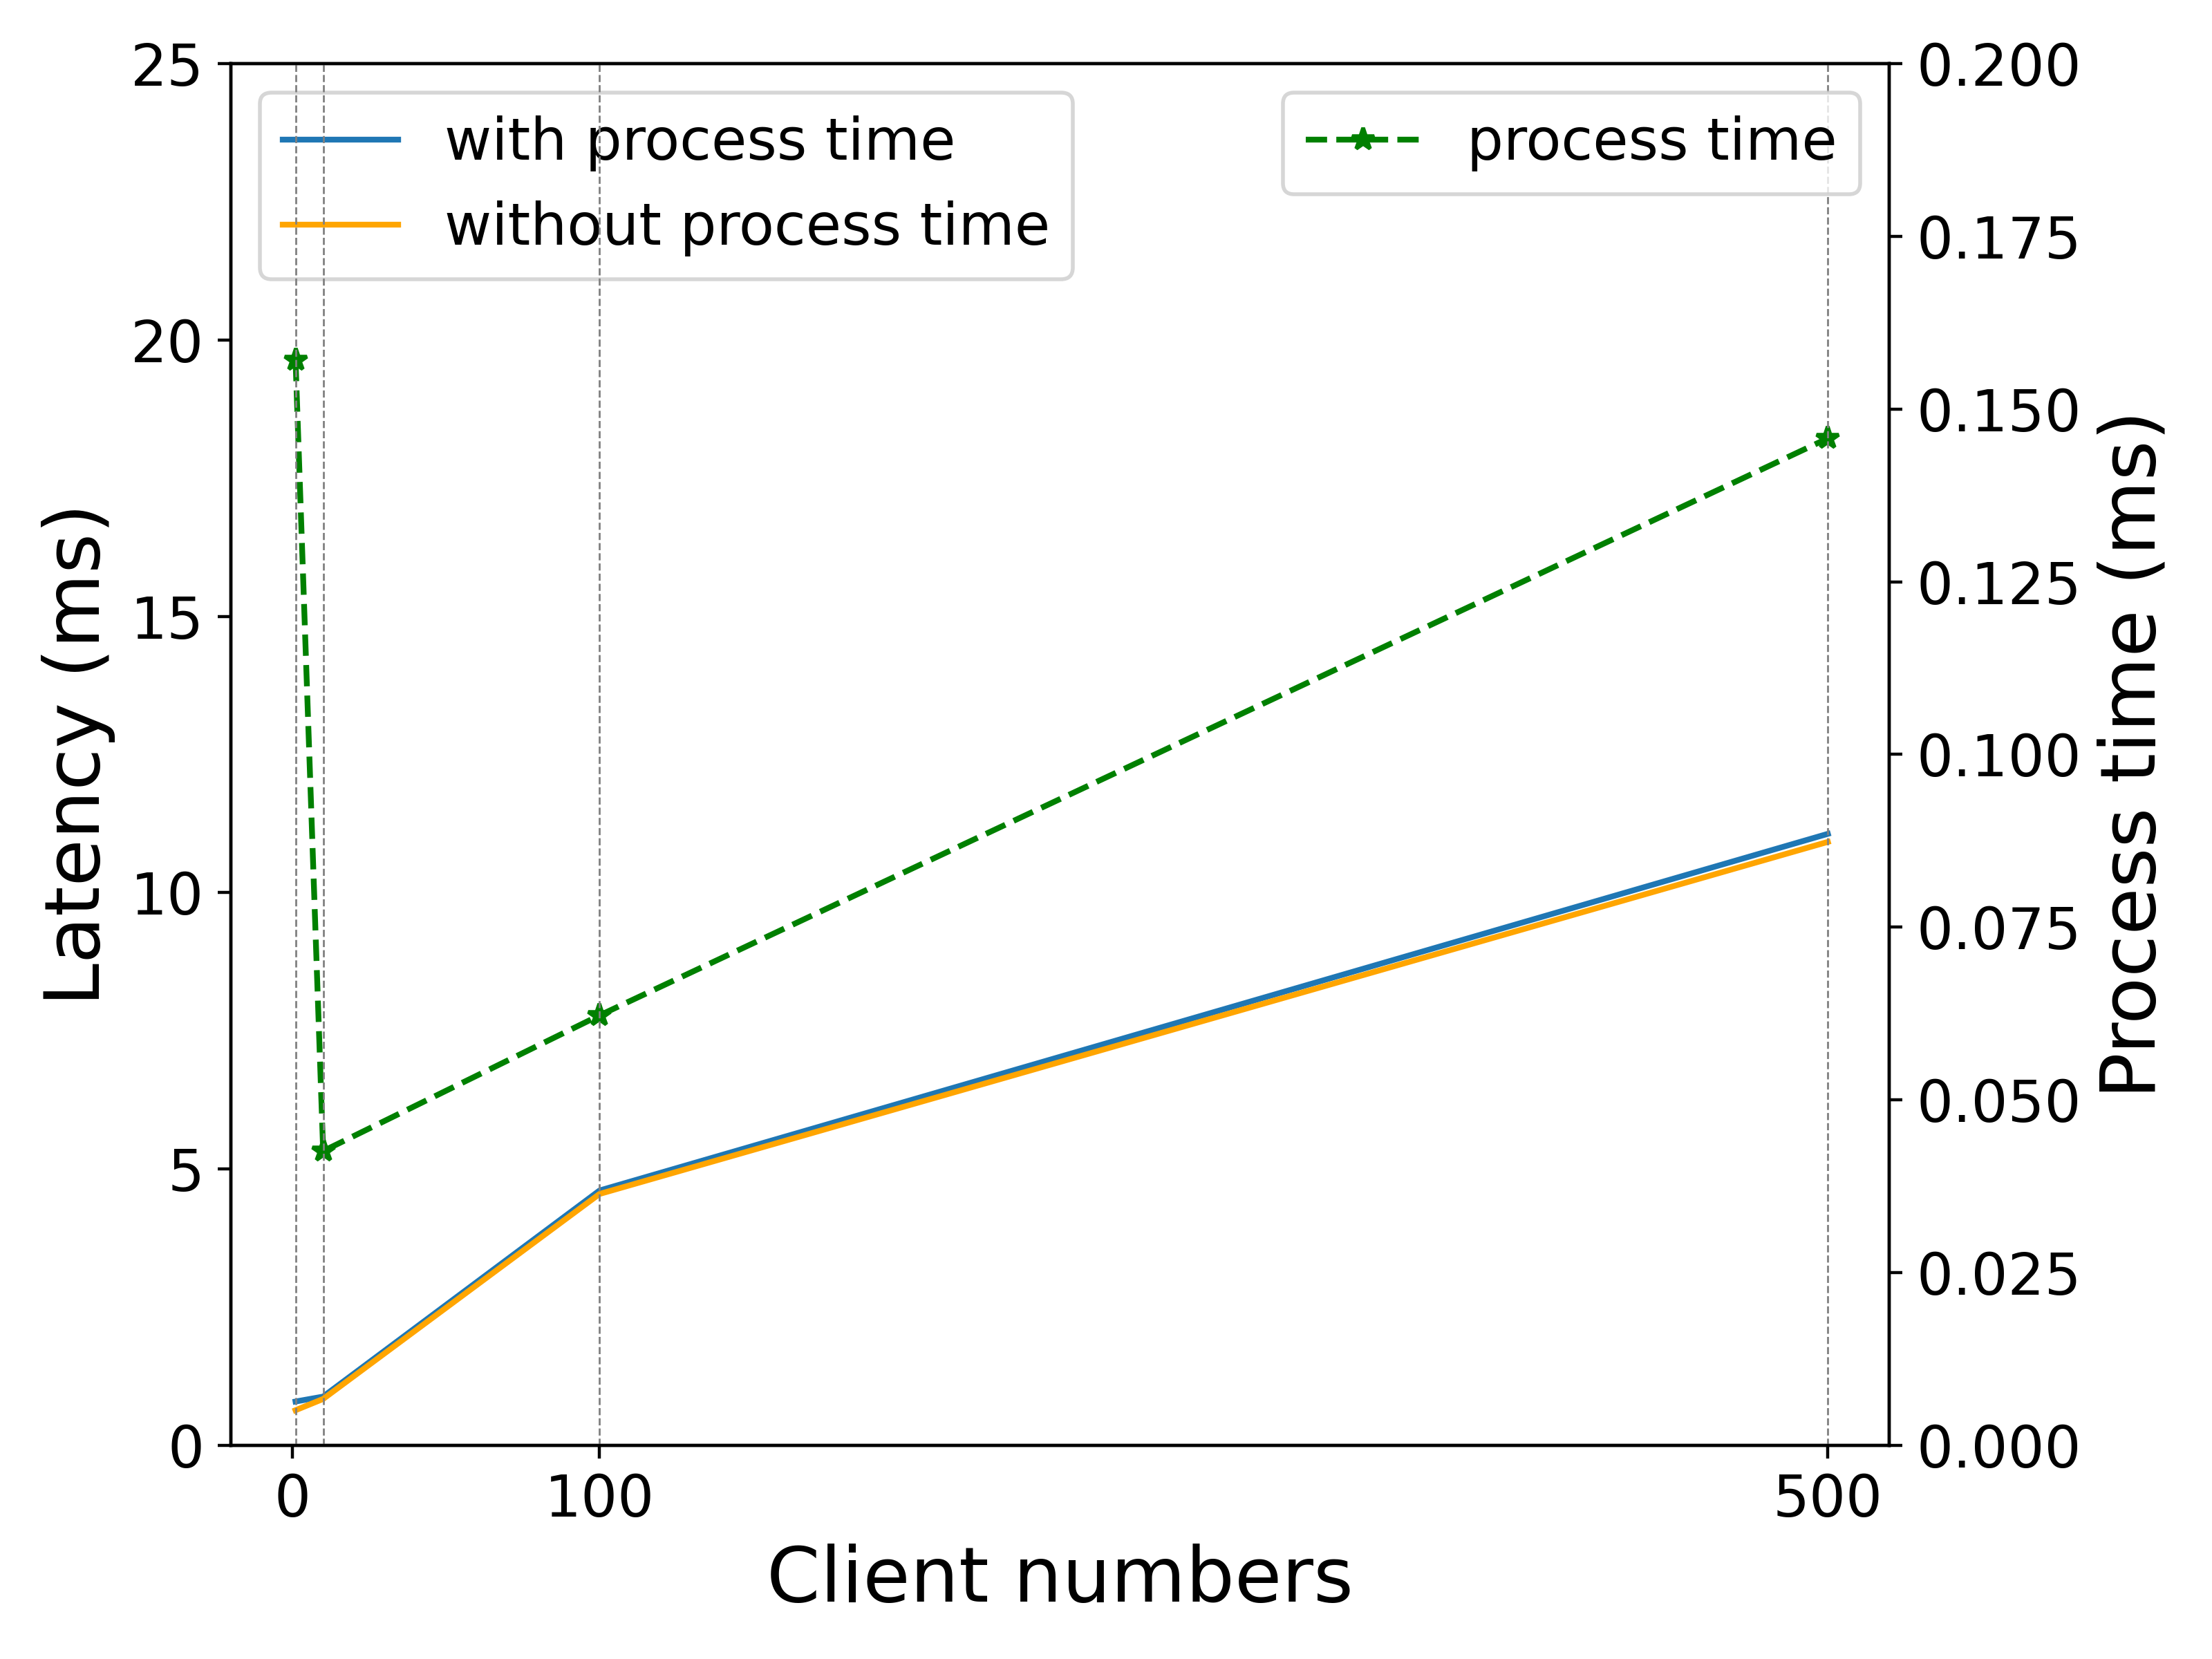
\includegraphics[width=.49\textwidth]{figures/tests/Average_string_messages_sending_time_of_100_tests_of_diff_client_numbers.png}\hfill 
    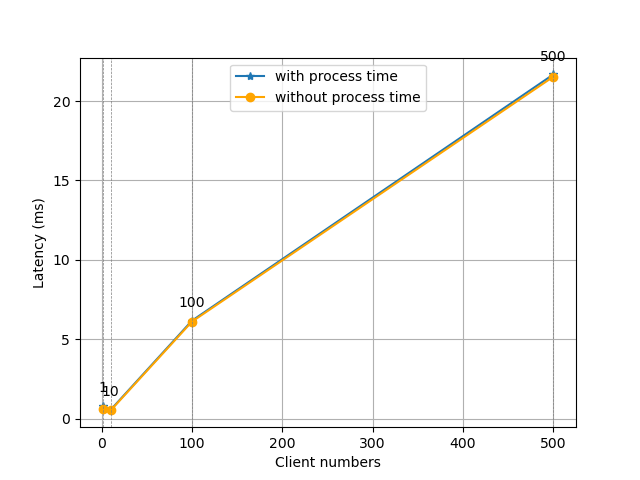
\includegraphics[width=.49\textwidth]{figures/tests/Average_string_messages_receiving_time_of_100_tests_of_diff_client_numbers.png}\hfill 
    \caption{Average delay of sending a string message 100 times 
    to a clientR from 1, 10, 100 or 500 clients separately. (a) Messages sent forward, 
    and (b) response messages from clientR. 
    \label{fig: proportional-clients}}
\end{figure}

By handling an increasing number of connection requests, and the growing demands 
of data processing capacity, the total delay with or without process time can be 
roughly described as an overall increasing process. However, it does not necessarily 
need to be linear due to the following reasons:  


\subsection{Test results of WebSocket and RESTful API} \label{chap: Result-RestFUL_WS}

\subsection{priority tests of WS server in diff. performance testing} \label{chap: Result-priority}

\section{External}\label{chap: Result-External}

\subsection{Test results of DTagents related to Azure Digital Twin} \label{chap: Result-DT}